%
%
%\citet{DAntona2000} presented the first hints the missing physics, well before the full severity of model deficiencies was understood. They showed that including a rudimentary prescription for the effects of magnetic fields on convection provided better...

Recently, our group demonstrated that magnetic fields may provide a viable explanation for observed surface-temperature dependent ages in young clusters and the discordance between HRD and MRD age estimates \citep[see Figure~\ref{fig:usco};][]{Feiden2016}. The hypothesis is that Lorentz forces generated by strong magnetic fields suppresses convective flows in young stars, which acts to cool the stellar surface \citep[e.g.,][]{DAntona2000, MM01, FC12b}. As a result, the contraction of young pre-main-sequence stars is delayed, meaning young stars have cooler temperatures and larger radii at a given age when magnetic inhibition of convection is included in model calculations \citep{MM10, Feiden2016}. The physical mechanism is analogous to formation of sunspots, where strong magnetic fields suppress convection causing the stellar plasma contained within a magnetic region to cool and thus appear darker than its surroundings \citep{Biermann1941, Deinzer1965}.

Previous investigations showed that magnetic inhibition of convection could relieve age discrepancies for the 25 Myr old $\beta$ Pictoris moving group \citep{MM10, Malo2014}. Ages inferred from the HRD of the $\beta$ Pictoris moving group using standard stellar evolution models indicated the group was 12 Myr old, while the same models provided an age of 20 Myr based on the lithium depletion boundary \citep{Someone2005, Binks2013}. However, by including magnetic inhibition of convection, \citet{MM10} and \citet{Malo2014} showed the two age estimates could be brought into rough agreement with an age between 25 -- 30 Myr. 

Magnetic models were successful at reconciling the two age estimates, but it was not clear whether the magnetic models were accurate because HRD and lithium depletion boundary studies are mass agnostic. To know whether magnetic models predict accurate properties for real stars, EBs in well-studied young clusters are needed. Masses and radii measured in EBs provide the most stringent tests of stellar models as mass is the primary model input and measured radii are more reliable than $T_{\rm eff}$ and luminosity estimates. In addition, finding EBs in young clusters would provide an opportunity to confirm the MRD age estimate against an age inferred from an HRD.

\begin{figure}
	\centering
    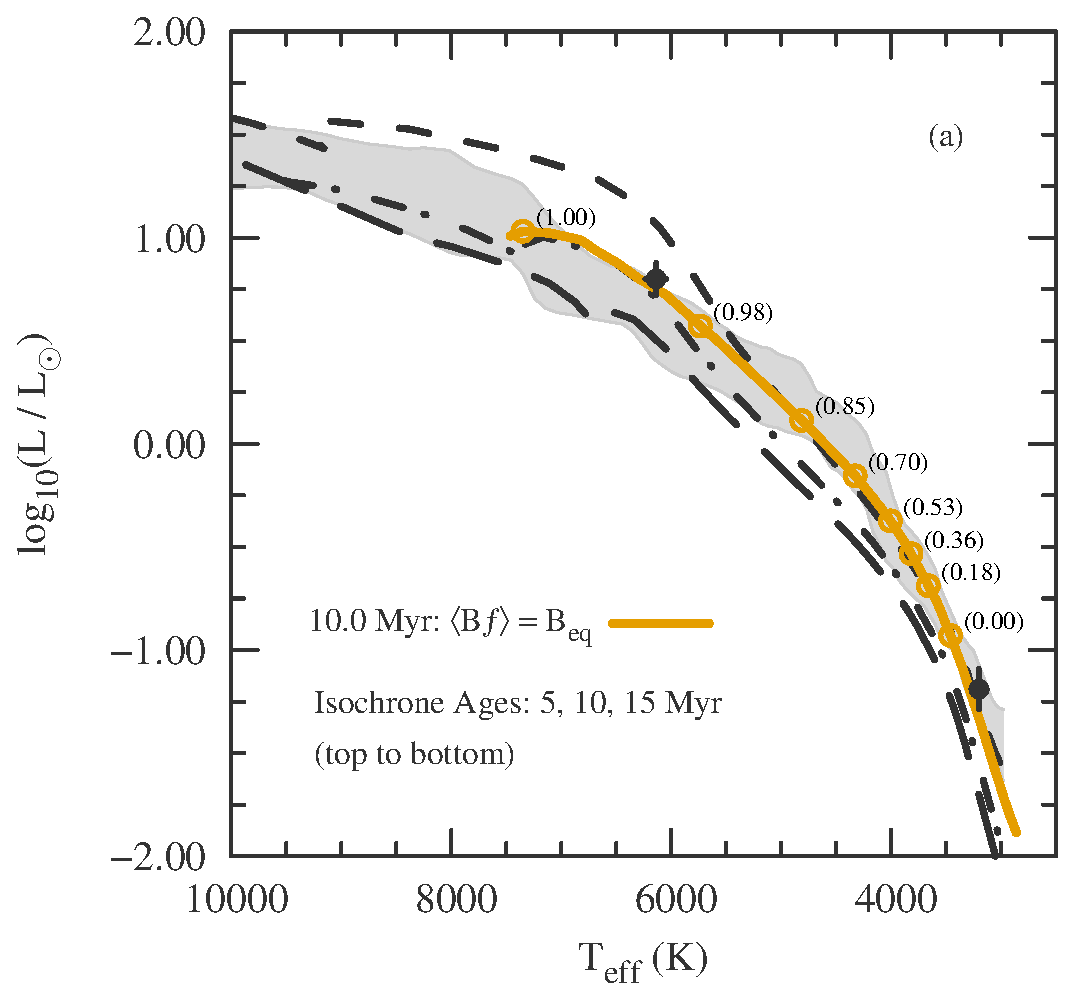
\includegraphics[scale=0.35]{fig/USco_HR_diagram.eps} \quad
    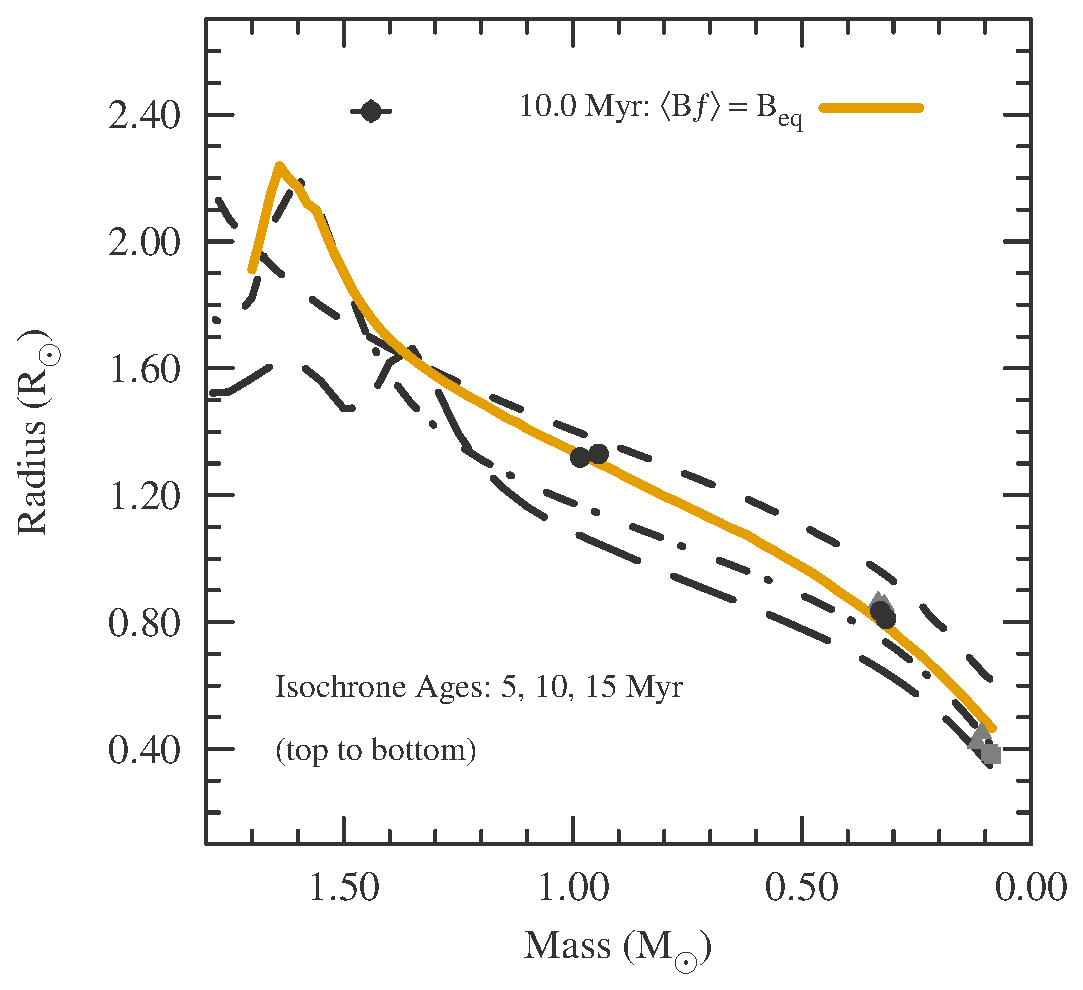
\includegraphics[scale=0.35]{fig/USco_MR_diagram.eps}
    \caption{({\it left}) HR diagram of Upper Scorpius with components of eclipsing binary systems UScoCTIO5 \citep{Kraus2015} and HD 144548 \citep{Alonso2015}
    observed by {\it Kepler}/K2 (black points). A 10 Myr magnetic stellar evolution isochrone is shown by the solid blue line. Note that the 10 Myr magnetic isochrone lies on top of the 5 Myr standard isochrone. ({\it right}) Mass-radius relationship for Upper Scorpius from {\it Kepler}/K2 eclipsing binary systems. {\it Unlike standard models, magnetic stellar evolution models naturally reproduce the slope of the low-mass mass-radius relationship at the same age predicted from the HR diagram.}}
    \label{fig:usco}
\end{figure}

A source of EBs in a well-studied young cluster became available when \kepler\ observed the Scorpius-Centaurus OB Association for 80 continuous days. A number of EBs were quickly identified, including two EBs for which precise masses and radii were determined \citep{Kraus2015, Alonso2015}. Critically, the two EBs occupied two distinct regions of the MRD, as shown in the right panel of Figure~\ref{fig:usco}. Comparing the mass-radius relation formed by these EBs, it is clear that standard models predict an incorrect slope for the mass-radius relationship and that the ages inferred from the MRD did not agree with ages inferred from the HRD.

We showed that including magnetic inhibition of convection in stellar models calculations produces 


The recent results of \citet{Feiden2016} are tantalizing, as they offer a path toward reliable young stellar ages, but important questions remain about the validity and accuracy of these ``magnetic stellar evolution models.'' First, properties of the magnetic field are prescribed in a rather ad-hoc fashion \citep{FC12b, FC13}. Simple functions are used to describe the magnetic field strength as a function of radius deep in a star \citep{FC13}, but the situation in real stars is far more complex and depends intimately on the precise structure and rotational velocity of the star \citep{Browning2008, Brown2010}. Second, the interaction of Lorentz forces on convection depend strongly on the magnetic field topology throughout the star \citep{FC13}. At the moment, models use a free parameter to describe an average magnetic field topology, but the parameter is fixed and not allowed to vary as would be expected for a real magnetic field \citep{FC12b}. Finally, the existing magnetic field framework requires the specification of the surface magnetic field strength \citep{FC12b}. This value is either chosen arbitrarily \citep{FC12b, FC13, FC14, FC14b}, or at best, order of magnitude estimates are used to describe a possible maximum value \citep{Feiden2016}. 

The full effect of these modeling choices are felt when stars are allowed to evolve in time. Properties of the magnetic field are a function of the stellar structure and stellar rotation, which both vary over time. Therefore, magnetic fields are expected to also evolve in time. These subtleties cannot be captured with existing magnetic model formulations and it remains unclear what the effect of an evolving magnetic field will have on stellar structure and evolution \citep{Feiden2016}. Ultimately, a complete description of how magnetic fields affect stellar structure would include a physical mechanism that relieves these ad-hoc prescriptions.

Describing how magnetic field generation depends on stellar structure and rotation is within the realm of magnetic dynamo theory. Dynamo theory describes the interaction between predominantly radial convective flows and azimuthal rotation, which are suitable for generating and sustaining magnetic fields. The general picture is that the poloidal component of the magnetic field is stretch into a toroidal configuration by latitudinally differential rotation ($\Omega$ effect) while turbulence associated with convection tends to stretch and twist the toroidal magnetic fields back into a poloidal component \citep[$\alpha$ effect; e.g.,][]{Parker1955}. The $\Omega$ effect are well established, but details of the $\alpha$ effect remain open to debate \citep{Pipin2012}. Nevertheless, simulations that model the formation and time evolution (over decade timescales) of magnetic fields are sufficiently mature to permit reliable estimates of the magnetic field strength and topology for a given star \citep{Brandenburg2012}.